\section{The State of TCDA: A Structured Literature Review}\label{sec:literature}

This section synthesises the current state of TCDA work, organised along
the taxonomy of \Cref{sec:framework}. We proceed chronologically through
three broad eras---early connections (2015--2019), methodological
advances (2020--2023), and application-driven work (2020--present)---and
close with a structured account of remaining gaps. The four seed works
of the field appear repeatedly as anchor citations: their role is to
show that the methodological building blocks of TCDA are already in
place and that the missing piece is the unifying framework we provide in
\Cref{sec:framework}. \Cref{fig:timeline} summarises the timeline.

% =====================================================================
% Figure: Parallel development timeline of TDA and CI with bridges
% Working draft -- user will refine final visual styling.
% =====================================================================
\begin{figure}[t]
\centering
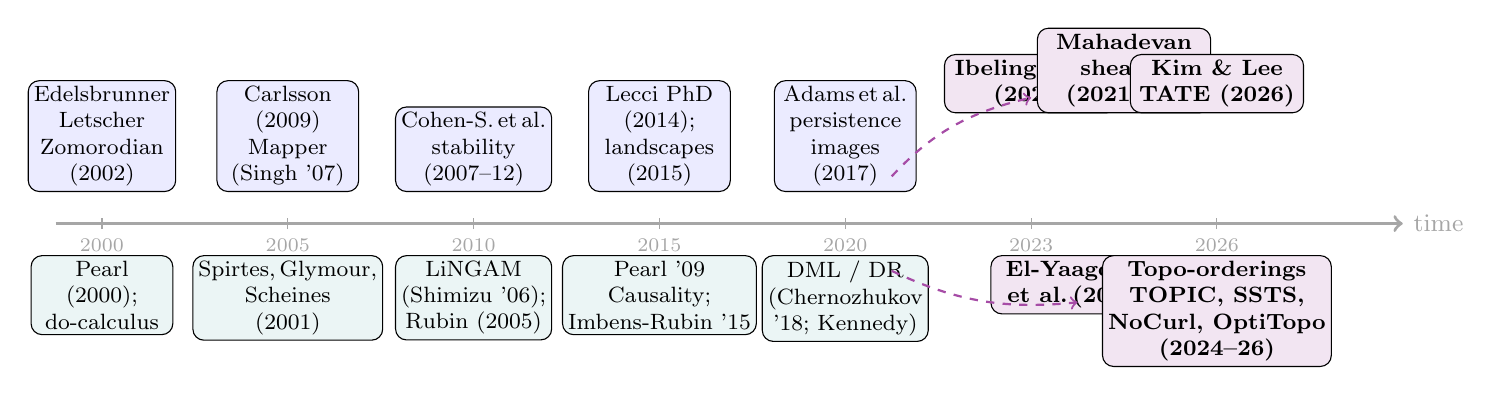
\begin{tikzpicture}[font=\footnotesize,
    yearnode/.style={draw, rounded corners, fill=blue!8, inner sep=2pt,
                     minimum width=18mm, align=center},
    cinode/.style={draw, rounded corners, fill=teal!8, inner sep=2pt,
                   minimum width=18mm, align=center},
    bridge/.style={draw, rounded corners, fill=violet!10, inner sep=2pt,
                   minimum width=22mm, align=center, font=\footnotesize\bfseries},
    xscale=1.18]
\draw[->, very thick, gray!70] (-0.5, 0) -- (14, 0)
  node[right, font=\small] {time};
\foreach \x/\y in {0/2000,2/2005,4/2010,6/2015,8/2020,10/2023,12/2026}{
  \draw[gray!70] (\x,-2pt) -- (\x,2pt) node[below=4pt, font=\scriptsize] {\y};
}
\node[yearnode, anchor=south] at (0,0.4)
  {Edelsbrunner\\Letscher\\Zomorodian\\(2002)};
\node[yearnode, anchor=south] at (2,0.4)
  {Carlsson\\(2009)\\Mapper\\(Singh '07)};
\node[yearnode, anchor=south] at (4,0.4)
  {Cohen-S.\,et\,al.\\stability\\(2007--12)};
\node[yearnode, anchor=south] at (6,0.4)
  {Lecci PhD\\(2014);\\landscapes\\(2015)};
\node[yearnode, anchor=south] at (8,0.4)
  {Adams\,et\,al.\\persistence\\images\\(2017)};

\node[cinode, anchor=north] at (0,-0.4)
  {Pearl\\(2000);\\do-calculus};
\node[cinode, anchor=north] at (2,-0.4)
  {Spirtes,\,Glymour,\\Scheines\\(2001)};
\node[cinode, anchor=north] at (4,-0.4)
  {LiNGAM\\(Shimizu '06);\\Rubin (2005)};
\node[cinode, anchor=north] at (6,-0.4)
  {Pearl '09\\Causality;\\Imbens-Rubin '15};
\node[cinode, anchor=north] at (8,-0.4)
  {DML / DR\\(Chernozhukov\\'18; Kennedy)};

\node[bridge, anchor=south] at (10,1.4)
  {Ibeling-Icard\\(2021)};
\node[bridge, anchor=south] at (11,1.4)
  {Mahadevan\\sheaves\\(2021--25)};
\node[bridge, anchor=south] at (12,1.4)
  {Kim \& Lee\\TATE (2026)};
\node[bridge, anchor=north] at (10.5,-0.4)
  {El-Yaagoubi\\et al.\,(2023)};
\node[bridge, anchor=north] at (12,-0.4)
  {Topo-orderings\\TOPIC, SSTS,\\NoCurl, OptiTopo\\(2024--26)};

\draw[->, dashed, thick, violet!70] (8.5,0.6) to[bend left=18] (10,1.6);
\draw[->, dashed, thick, violet!70] (8.5,-0.6) to[bend right=18] (10.5,-1.0);
\end{tikzpicture}
\caption{Parallel development of TDA (upper band, blue) and causal
inference (lower band, teal) with emerging bridges (violet) in the
2020s. Until $\sim$2020 the two communities developed largely
independently---TDA building from persistence and stability towards a
statistical-inference programme \citep{edelsbrunner2002topological,
carlsson2009topology,cohen2007stability,lecci2014statistical,
adams2017persistence}, while causal inference matured under the Pearl
and Rubin programmes and absorbed double-machine-learning
\citep{pearl2009causality,imbens2015causal,chernozhukov2018double}.
The bridge papers of 2021--2026---topology on the space of SCMs
\citep{ibeling2021topological}, sheaf-theoretic causal calculi
\citep{mahadevan2025sheaf}, topological treatment effects
\citep{kim2026topological}, simulation-based TDA inference for
multivariate time series \citep{elyaagoubi2023statistical}, and
topological-ordering algorithms for causal discovery
\citep{tran2024constraining,xu2025information,nocurl2024,
wu2026optimization}---together delineate the TCDA programme.}
\label{fig:timeline}
\end{figure}


\subsection{Early connections (2015--2019)}\label{sec:lit_early}

The pre-2020 period saw TDA and causal inference develop largely
independently. Three threads, however, foreshadow TCDA: the maturation
of statistical TDA, the rise of topological approaches in
causal-adjacent applications (brain networks, dynamical systems), and
isolated calls for category-theoretic foundations on both sides.

\paragraph{Statistical TDA matures.}
By 2014, the date of \citet{lecci2014statistical}'s PhD thesis-scale
treatise, persistent homology had moved from algebraic topology and
computational geometry into the statistical mainstream. Foundational
algorithmic work \citep{edelsbrunner2002topological,zomorodian2005topology,
zomorodian2005computing} was complemented by a wave of inferential
results: confidence sets for persistence diagrams via the bottleneck
bootstrap \citep{fasy2014confidence,chazal2013bootstrap}; rates of
convergence for the persistent homology of samples
\citep{chaudhuri2010rates,chazal2015optimal}; Banach-space-valued
landscapes that admit a functional central limit theorem
\citep{bubenik2015statistical,chazal2014stochastic,lecci2014statistical};
and probability distributions on the space of diagrams \citep{mileyko2011probability,
turner2014frechet}. \citet{lecci2014statistical} is the most
comprehensive PhD-thesis-scale synthesis of this material; the
inferential machinery it organises---confidence sets, hypothesis tests,
bootstrap, rates---is the statistical scaffolding that any subsequent
TCDA estimator inherits. The introduction of persistence images
\citep{adams2017persistence}, PerLay neural layers
\citep{carriere2020perslay}, and PLLay \citep{kim2020pllay} closed the
gap towards machine-learning workflows, and stability arguments for
the silhouette \citep{chazal2014stochastic} pre-figured the
silhouette-based causal contrast of \citet{kim2026topological}.

\paragraph{Topological brain networks: causal-adjacent but not causal.}
Network neuroscience absorbed TDA early. The Bullmore-Sporns programme
\citep{bullmore2009complex,sporns2013structure,bassett2009human} cast
brain connectivity as a graph, and TDA naturally lifted the discussion
from graphs to higher-order simplicial structures
\citep{sizemore2018cliques,sizemore2019importance}. Cliques and cavities
in the human connectome were shown to organise functional integration
and segregation
\citep{sizemore2018cliques}; small-world propensity was
re-cast as a topological invariant \citep{muldoon2016small}; and trends
in topological summaries of EEG/MEG across cognitive states began to
serve as quantitative biomarkers \citep{fathian2022trend,
gorrostieta2018time}. None of this work was framed in causal terms.
\citet{friston2011functional}'s functional and effective connectivity
agenda was the closest causal counterpart, but it operated in a
parametric (state-space, DCM) framework that did not interact with
topology. The seeds of D1 (TCDA for time-series causality) and C1
(Betti numbers as causal explanation) of \Cref{sec:framework} are here
visible in embryonic form.

\paragraph{TDA for time series and dynamical systems.}
The other natural site of TDA-causality interaction is dynamical
systems: cycles in $\PHk{1}$ of a Takens reconstruction correspond to
recurrent or periodic behaviour. \citet{chung2009persistence,
pachauri2011topology} applied persistence to medical-image time series;
\citet{umeda2017time,kim2018time} used PH features for time-series
classification; \citet{gholizadeh2018short} surveyed the field. Stability
of persistence under filtration deformation
\citep{cohen2007stability,chazal2016structure} ensured that the
features used were not noise artefacts. Crucially, these works treated
PH as a \emph{descriptive} statistic; the next step---using PH inside a
causality test---came after 2020 and is reviewed in
\Cref{sec:lit_method}.

\paragraph{Categorical and sheaf-theoretic preludes.}
On the structural side, \citet{spivak2014category,curry2014sheaves,
robinson2014topological,robinson2014hypothesis} developed category-
theoretic and sheaf-theoretic vocabularies for data analysis,
emphasising functoriality and gluing. Independently, Pearl's
\citep{pearl1995causal,pearl2009causality} programme had been re-cast
in terms of categories of structural equation models, and
\citet{galles1998axiomatic} provided axiomatic foundations for
counterfactuals. \citet{henry2020bridging} explicitly argued that
bridging the two would require new structural primitives. None of
these papers connected TDA to causal inference; together they prepared
the categorical vocabulary that the Mahadevan programme would later
deploy.

\paragraph{Causal-inference foundations that TCDA will inherit.}
Concurrent with the TDA timeline, the causal-inference community
consolidated around three programmes: Pearl's structural-causal-models
and do-calculus \citep{pearl1995causal,pearl2009causality,pearl2018book};
Rubin's potential outcomes \citep{rubin1974estimating,rubin2005causal,
imbens2015causal}; and the constraint-based and score-based discovery
algorithms \citep{spirtes2001causation,meek1995strong,peters2014causal,
shimizu2006lingam}. A separate inferential thread on identification
\citep{tian2000probabilities,tian2002general,avin2005identifiability}
established the language in which any TCDA solution must ultimately be
phrased. The doubly-robust efficient-estimation programme
\citep{robins1989probability,chernozhukov2018double,kennedy2016semiparametric}
would, in turn, supply the AIPW machinery that \citet{kim2026topological}
extend to the topological setting in 2026.

The picture by 2019 is clear: both fields are mathematically and
statistically mature; both have begun to be applied to the same
empirical objects (brain networks, time series, cosmological structure);
and yet no formal bridge yet exists. The four seed papers of the field
all appear within the next four years.

\subsection{Methodological advances (2020--2023)}\label{sec:lit_method}

Between 2020 and 2023 the bridge formed. Five sub-threads emerged in
near-simultaneous fashion: (i)~the topology of the space of structural
causal models; (ii)~category-theoretic and sheaf-theoretic causal
calculi; (iii)~topology-based causal discovery via ordering; (iv)~causal
treatment effects defined directly on topological summaries; and
(v)~topological deep learning with explicit causal applications.

\paragraph{The topology of SCMs.}
\citet{ibeling2021topological} is the methodological pivot for Domain B
of \Cref{sec:framework}. The authors equip the space $\mathfrak{M}$ of
structural causal models with a family of topologies that mirror the
Pearl--Bareinboim causal hierarchy: the observational topology refines
to an interventional topology and then to a counterfactual topology.
The central theorem---a topological no-free-lunch result---states that
the subset of $\mathfrak{M}$ on which assumption-free causal inference is
possible is \emph{topologically meagre} (in the sense of Baire). Two
classical traditions converge here. The first is the measure-theoretic
no-free-lunch programme of \citet{oxtoby1971measure,belot2020absolutely};
the second is the topology-of-statistical-verifiability programme of
\citet{dembo1994topological,genin2017topology,genin2018topology,
genin2020statistical,genin2021statistical}, which shows that open sets
in the weak topology correspond to verifiable statistical hypotheses.
\citet{ibeling2021topological} lifts both to the causal hierarchy and
provides accommodation for SCMs over countably-infinite variable sets
via Borel-product topologies. The companion identifiability papers
\citep{ibeling2019open,ibeling2020probabilistic} complete the picture.
For TCDA, the result is foundational: it tells us that the search for a
causal answer in the absence of topological structure on the model
space is a search in a meagre set, and that topology is the right
language for the negative results of the field.

\paragraph{Sheaf and topos foundations.}
A parallel programme, anchored in \citet{mahadevan2021causal,
mahadevan2022universal,mahadevan2025sheaf}, recasts causal inference as
a universal construction in a topos of sheaves over a base category of
contexts. Do-calculus is recovered through the subobject classifier;
identification becomes a sheaf-cohomological obstruction; the standard
exchangeability/positivity/consistency triple is interpreted as
descent conditions. This work realises B3 (functorial causal inference)
of \Cref{sec:framework} and connects it to the broader categorical
data-analysis programme of \citet{spivak2014category,curry2014sheaves,
hajij2023topological,papamarkou2024position}.
The Alexandroff-topology approach of \citet{willig2025alexandroff}
provides a more elementary entry point and recovers parts of the
Ibeling-Icard hierarchy as Alexandroff specialisations.

\paragraph{Topology-based causal discovery: ordering algorithms.}
A different methodological thread takes the ordering of nodes in a
causal DAG to be the primary object and infers it via topological or
information-theoretic means. The score-based ordering of
\citet{rolland2022score} uses the Hessian of the log-density to
extract a topological order under additive-noise assumptions and was
followed by a wave of related work: TOPIC
\citep{tran2024constraining} uses topological-order constraints in a
DAG-learning loss; SSTS \citep{xu2025information} adapts the order to
sequential and stochastic time-series; NoCurl-X
\citep{nocurl2024} uses the Hodge decomposition of a $1$-chain on the
candidate DAG to extract the harmonic (acyclic) component; OptiTopo
\citep{wu2026optimization} optimises over topological orders directly;
CaPS \citep{rolland2022score} originally introduced the score-Jacobian
formulation. Hodge-decomposition methods more generally
\citep{desilva2007coverage} ground the gradient/curl/harmonic split
that we exploit in C2 (persistent cohomology for mediation analysis).
In the language of \Cref{prop:identifiability}, this entire thread
selects a different topological functor $\Tc$ and asks when the
$G \mapsto \Tc(\mathcal{P}_G)$ map is injective on a class of admissible
graphs.

\paragraph{Treatment effects as topological functionals.}
\citet{kim2026topological} is the methodological pivot for Domains A3
and B1. The authors define the \emph{topological average treatment
effect}
\[
  \TATE = W_1\!\bigl(\Dgmk{k}(P^{a=1}),\,\Dgmk{k}(P^{a=0})\bigr)
\]
and a closely related power-weighted-silhouette contrast, develop a
doubly-robust AIPW estimator with a $\sqrt n$-rate under product-rate
nuisance conditions, prove weak-convergence guarantees in the space of
silhouette functions, supply a $W_1$-based stability bound that links
1-Wasserstein perturbations of the diagram to sup-norm perturbations
of the silhouette, and demonstrate the methodology on SARS-CoV-2 CT
scans \citep{soares2020sars} and the GEOM-Drugs molecular-graph
database \citep{axelrod2022geom}. The work is the first to combine all
three ingredients of TCDA in one estimator: a non-Euclidean outcome
space ($\Mc$ = a space of distributions over diagrams), a topological
functor $\Tc = \varphi(\cdot;r)$, and a causal query $\Cc$ with
calibrated uncertainty. \citet{saki2026beyond} extends the topological-
contrast idea ``beyond the silhouette'' to more general functional
summaries; \citet{ballester2026topological} develops complementary
representations; \citet{deepcausalitytopology2026} connects the
construction to deep causal models. The geodesic-ATE programme of
\citet{kurisu2024geodesic} for Riemannian-valued outcomes is a sister
contribution that places non-Euclidean potential outcomes on the same
footing without invoking persistence.

\paragraph{Simulation-based inference and dependence networks.}
\citet{elyaagoubi2023statistical} addresses an under-served methodological
problem: how to evaluate TDA-based inference for multivariate time
series when no ground truth is available. The authors construct a
generative model---mixtures of latent AR(2) processes---that allows
researchers to \emph{prescribe} the number of cycles in the dependence
network, and they use this to test hypotheses about the resulting
$\PHk{1}$. \citet{elyaagoubi2023topological} extends the construction to
asymmetric dependence. Together these papers anchor D1 (time-series
causality) of \Cref{sec:framework} and provide benchmarking
infrastructure that the rest of the field can adopt.

\paragraph{Topological deep learning and topological regularisation.}
A fifth thread brings topology into representation learning. PerLay
\citep{carriere2020perslay} and PLLay \citep{kim2020pllay} are
differentiable persistence layers that allow gradient-based learning
on diagrams; the topological-deep-learning survey of
\citet{hajij2023topological} consolidates the area, and
\citet{papamarkou2024position} argues for its centrality going forward.
\citet{farzam2025topology} uses topological summaries as
regularisers in causal-representation models, demonstrating robustness
under heavy-tailed noise. \citet{xu2021topological} introduces
topological invariants in deep generative models with causal
structure. \citet{guan2025causal} and \citet{ma2025causal} extend
these ideas to causal disentanglement.

The methodological state by 2023 is therefore that every component of
\Cref{def:tcda}---a topological space $\Mc$ of observations, a causal
graph $G$, a topological functor $\Tc$, and a causal query $\Cc$---is
addressable by at least one well-developed line of research. What is
missing is the joint study.

\subsection{Application-driven work (2020--present)}\label{sec:lit_app}

The 2020--present period saw rapid uptake of TDA in scientific
application areas where causal questions are central. We organise the
account by domain.

\paragraph{Healthcare, drug discovery, and biomedicine.}
TDA of biological structure has a long pedigree \citep{kasson2007persistent,
chung2009persistence}, but causal questions became central only
recently. Persistent homology of protein conformations
\citep{kovacev2016using,cang2018integration} identifies binding-site
topology that responds to ligand intervention---an instance of the
TATE-style contrast in \citet{kim2026topological}, who explicitly use
the GEOM-Drugs molecular-graph database \citep{axelrod2022geom} to
demonstrate that ligand-binding induces topological change. CT-image
analysis of SARS-CoV-2 \citep{soares2020sars,iqbal2025classification}
constructs cubical persistent homology from imaging data and feeds the
resulting summary into classification and treatment-effect estimators;
\citet{kim2026topological} use the same dataset as one of two
methodological case studies. Topological feature extraction in tumour
classification \citep{iqbal2025classification} and disease-progression
modelling on cell-type manifolds
\citep{kim2018topological,carlsson2020topological,corcoran2023topological}
exemplifies the C3 (stratified heterogeneity) and D3 (industry
applications) face of \Cref{sec:framework}. A central remaining issue,
which \Cref{sec:research} treats as an open question, is identifiability
when topological biomarkers are derived from imaging modalities subject
to scanner and protocol drift.

\paragraph{Neuroscience and cognitive science.}
The brain-network literature \citep{bullmore2009complex,bassett2009human,
sporns2013structure,muldoon2016small,sizemore2018cliques,
sizemore2019importance,fathian2022trend} is the densest application
site for sub-domain C1 (Betti numbers as causal explanation): a
persistent $1$-cycle in the functional Granger network of a healthy
brain has been linked to re-entrant cortical loops that
disease---epilepsy, Alzheimer's, schizophrenia---perturbs. Spectral and
graphical extensions \citep{ombao2022spectral,gorrostieta2018time}
sharpen the picture. The simulation framework of
\citet{elyaagoubi2023statistical} ties the empirical literature back to
a controlled testbed: researchers can prescribe how many cycles a
generative model produces and check that a TDA discovery method
recovers them.

\paragraph{Climate, cosmology, and Earth science.}
Persistent homology of cosmological density fields
\citep{sousbie2011persistent,vandeweygaert2011alpha,
cisewski2014nonparametric} established the descriptive template for
spatial TDA, and recent applications transfer this template to climate
weather regimes \citep{strommen2025topological,smith2025multiscale,
smith2025harnessing}. The causal questions in this domain---attribution
of an extreme-precipitation event to a Pacific oscillation, attribution
of regime change to anthropogenic forcing---are precisely the
spatiotemporal causal contrasts of sub-domain D2. To date, however, the
TDA and the attribution communities have proceeded largely in parallel;
the explicit TCDA pairing of $(\Mc, G, \Tc, \Cc)$ in climate science is
nascent.

\paragraph{Finance and economics.}
\citet{gidea2018topological,ismail2022early} apply persistent-landscape
analysis to financial time series and demonstrate that
topological summaries serve as early-warning signals of crashes. The
causal content---attribution of a regime change to a triggering market
factor---is implicit in their construction but not formally tested.
\citet{leykam2023topological} review the broader topological-finance
literature.

\paragraph{Time-series and dynamical-system causality.}
\citet{bando2022causal} combine persistent homology of Takens
embeddings with convergent cross mapping to extract dynamical causal
links between coupled oscillators; \citet{harnack2017causal,
gholizadeh2018short} use persistence to augment Granger-type tests.
\citet{krasnovsky2025causal} extends this to multivariate stochastic
systems with structural breaks. The combination directly instantiates
the sub-domain D1 picture: $\Tc = \PHk{1}$ of a Takens embedding;
$G$ = Granger graph; $\Cc$ = a causal hypothesis test.

\paragraph{Materials and physical sciences.}
TDA in materials science \citep{nigmetov2022topological} and topological
photonics \citep{leykam2023topological} pose causal questions about
structure--property relationships. The TCDA tuple here selects
$\Mc = $ a configuration space of atomic structures, $\Tc = \PHk{0,1,2}$
on the Vietoris-Rips filtration of atomic positions, and $\Cc$ a
causal regression of property on structure mediated by topological
features. This is one of the most natural application domains and is
explicitly identified in \Cref{sec:research}.

\subsection{Gaps in the current literature}\label{sec:lit_gaps}

Five gaps recur across the threads surveyed above. Each motivates a
specific open question or research avenue in \Cref{sec:research}.

\paragraph{Absence of a unified framework.}
The five methodological threads of \Cref{sec:lit_method} fix different
corners of the TCDA tuple but do not interact. \citet{ibeling2021topological}
study topology on $\mathfrak{M}$ but not topological summaries of data;
\citet{kim2026topological} study topological summaries of data but treat
$\mathfrak{M}$ as fixed; \citet{mahadevan2025sheaf} build the
categorical scaffolding without explicit persistence-stability
results; \citet{elyaagoubi2023statistical} provide benchmarks without a
universal causal query. Our \Cref{def:tcda} is the proposed unifier.

\paragraph{Computational and software fragmentation.}
TDA libraries (\texttt{Ripser} \citealp{bauer2021ripser};
\texttt{GUDHI} \citealp{gudhi2021}; \texttt{giotto-tda}
\citealp{tauzin2021giotto}) and causal-inference libraries (\texttt{DoWhy},
\texttt{causal-learn}, \texttt{EconML}) do not interoperate; converting
a persistence diagram into a causal-effect estimand requires custom
plumbing. \Cref{sec:research} lists this as Computational Challenge~C3.

\paragraph{Missing benchmark datasets.}
Causal-discovery benchmarks (CMU-CausalDisco, the CausalBench suite of
\citealp{causaldisco2023survey,timeseriescd2023}) do not include
topological structure as a controlled covariate; conversely,
TDA benchmarks do not encode causal mechanisms. The simulation framework
of \citet{elyaagoubi2023statistical} is the closest analogue but is
restricted to time-series dependence networks; a more general TCDA
benchmark suite is one of the most actionable contributions a community
project could make.

\paragraph{Theoretical disconnect between functorial and methodological threads.}
The Mahadevan sheaf programme \citep{mahadevan2021causal,
mahadevan2022universal,mahadevan2025sheaf} has not yet been used to
analyse the AIPW estimator of \citet{kim2026topological}; conversely,
the Kim-Lee stability theorem has not been re-derived as a
sheaf-cohomological obstruction. The two halves of the field speak
different languages and the dictionary remains to be written. Several
open questions in \Cref{sec:research} (Q3, Q4, Q7) target precisely
this disconnect.

\paragraph{Absence of formal causal interpretation for topological features.}
The brain-network and finance literatures freely use phrases like
``a 1-cycle indicates a feedback loop'' \citep{sizemore2018cliques,
elyaagoubi2023statistical} or ``a persistent crash signature
identifies a regime shift'' \citep{gidea2018topological,
ismail2022early}, but in neither case is the causal interpretation
formally tied to an intervention. Sub-domain C1 of \Cref{sec:framework}
exists precisely because the field has not yet articulated a principled
language for assigning causal semantics to topological features.
\Cref{sec:research} formalises this as Open Question Q5.

\medskip
The methodological building blocks of TCDA are therefore in place; what
the field lacks is the joint formulation, the calibrated estimators,
the interoperable software, the benchmark suites, and the explicit
causal interpretive overlay on topological features.
\Cref{sec:case_studies,sec:research} take these gaps as the starting
point for the agenda we propose.
